% Task 1
\newpage
\section*{Task 1}

In this section, a state machine will be 
developed for controlling the switching
on and off of two pumps, to fill a tank.
The are controlled by two sensors from 
the upper part of the tank (S) and the 
lower part of the tank (I). The actions
to take are as follows:

\begin{itemize}
    \item Tank full: S = I = 1 - Pumps OFF
    \item Tank empty: S = I = 0 - Pumps ON
    \item Half full tank: S = 0 \& I = 1 - Pumps alternate 
\end{itemize}

With this in mind, a Moore machine is 
developed as follows.

\begin{figure}[H]
    \begin{centering}
    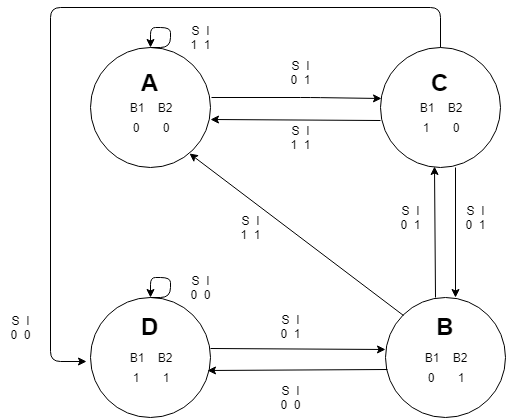
\includegraphics[width=0.75\textwidth]{data/Graficos1/1a_fsm.png}
    \par\end{centering}
    \caption{Moore state machine diagram}
\end{figure}

Using two bits to asign the states, a table 
of transitions is made, as shown below.

\begin{figure}[H]
\begin{centering}
\begin{tabular}{|c|c|c|c|c|c||c|c|}
    \hline 
    \multicolumn{2}{|c|}{Estado Actual} & \multicolumn{4}{c||}{Estado Siguiente} & \multicolumn{2}{c|}{Salidas}\tabularnewline
    \hline 
    \hline 
    \multirow{2}{*}{} & \multirow{2}{*}{y2 - y1} & \multicolumn{4}{c||}{S - I} & \multirow{2}{*}{B1} & \multirow{2}{*}{B2}\tabularnewline
    \cline{3-6} 
     &  & 00 & 01 & 10 & 11 &  & \tabularnewline
    \hline 
    A & 00 & X & C & X & A & 0 & 0\tabularnewline
    \hline 
    B & 01 & D & C & X & A & 0 & 1\tabularnewline
    \hline 
    C & 10 & D & B & X & A & 1 & 0\tabularnewline
    \hline 
    D & 11 & D & B & X & X & 1 & 1\tabularnewline
    \hline 
    \end{tabular}
    \caption{Moore state machine - Transitions}
\end{centering}
\end{figure}

\newpage

From the table, using Karnaugh's maps (see resolution in $Annex$) the 
functions for the state variables and the 
two pumps outputs result as shown below.
$$Y_2 = \overline{I} + \overline{S} \cdot \overline{y_2}$$ 
$$Y_1 = \overline{I} + \overline{S} \cdot y_2$$ 
For the outputs, $B_1 = y_2$ and $B_2 = y_1$.  
Finally, the state machine is implemented using 
D Flip Flops:

\begin{figure}[H]
    \begin{centering}
    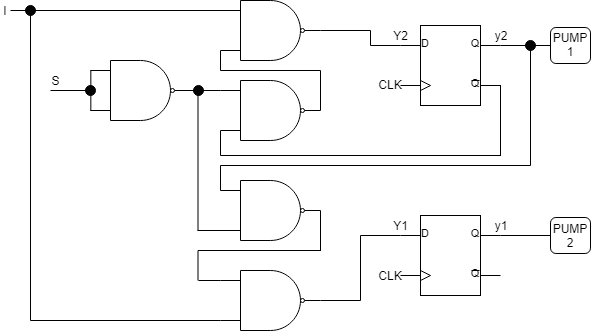
\includegraphics[width=0.6\textwidth]{data/Graficos1/1a_Compuertas_Moore.png}
    \par\end{centering}
    \caption{Moore state machine - Circuit implementation}
\end{figure}

On the other side, the same system is implemented 
now using a Mealy state machine, as shown below.

\begin{figure}[H]
    \begin{centering}
    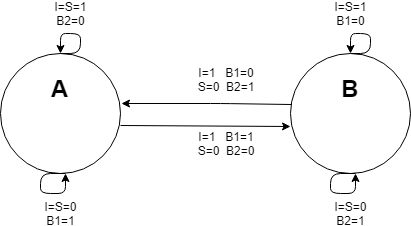
\includegraphics[width=0.5\textwidth]{data/Graficos1/1b_fsm.png}
    \par\end{centering}
    \caption{Mealy state machine diagram}
\end{figure}

Notice that the direct connection between the 
input and the pumps outputs reduces the number 
of states from four to two, in comparison with 
the Moore machine.
Using one bit for the states, a table of transitions
is made as follows.

\begin{figure}[H]
\begin{centering}
\begin{tabular}{|c|c|c|c|c|c||c|c|c|c|}
    \hline 
    \multicolumn{2}{|c|}{Estado Actual} & \multicolumn{4}{c||}{Estado Siguiente} & \multicolumn{4}{c|}{Salidas}\tabularnewline
    \hline 
    \hline 
    \multirow{3}{*}{} & \multirow{3}{*}{y} & \multicolumn{4}{c||}{S - I} & \multicolumn{4}{c|}{S - I}\tabularnewline
    \cline{3-10} 
     &  & 00 & 01 & 10 & 11 & 00 & 01 & 10 & 11\tabularnewline
    \cline{3-10} 
     &  & \multicolumn{4}{c||}{y} & B1 - B2 & B1 - B2 & B1 - B2 & B1 - B2\tabularnewline
    \hline 
    A & 0 & A & B & A & X & 11 & 10 & XX & 00\tabularnewline
    \hline 
    B & 1 & B & A & B & X & 11 & 01 & XX & 00\tabularnewline
    \hline 
    \end{tabular}
    \caption{Mealy state machine - Transitions}
\end{centering}
\end{figure}

Using again Karnaugh's maps (see resolution in $Annex$), the resulting functions for
the state variable and the two pumps outputs are shown below.
$$Y = \overline{y} \cdot \overline{S} \cdot I + y \cdot \overline{I} + y \cdot S$$ 
$$B_1 = \overline{y} \cdot \overline{S} + \overline{S} \cdot \overline{I}$$
$$B_2 = \overline{S} \cdot \overline{I} + y \cdot \overline{S}$$
Finally, the state machine is implemented using
one D Flip Flop.

\begin{figure}[H]
    \begin{centering}
    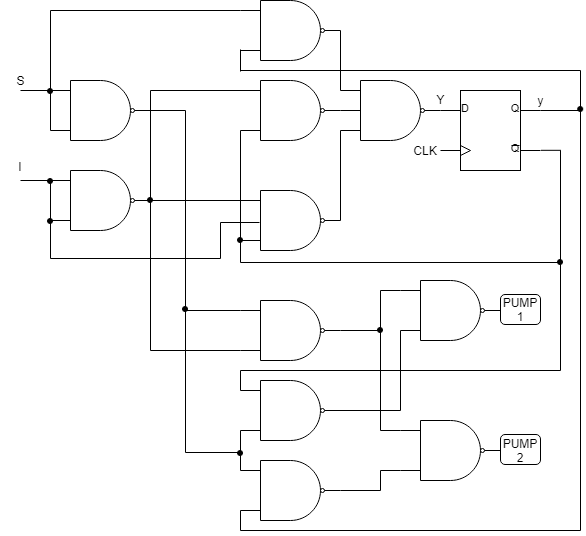
\includegraphics[width=0.6\textwidth]{data/Graficos1/1b_Compuertas_Mealy.png}
    \par\end{centering}
    \caption{Mealy state machine - Circuit implementation}
\end{figure}

\subsection *{Verilog tests}
This task was tested using verilog tests benchs. Here we show the results of simulating Moore's and Mealy's implementations.
For extra support, it was also simulated on Proteus.

\begin{figure}[H]
    \begin{centering}
    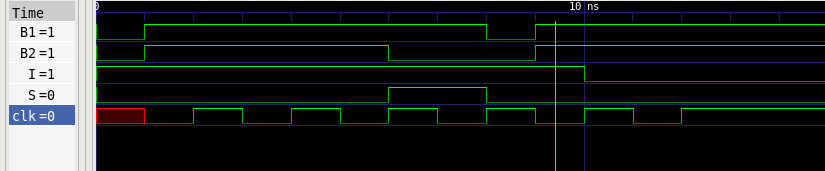
\includegraphics[width=0.7\textwidth]{data/Graficos1/ej1b.png}
    \par\end{centering}
    \caption{Moore state machine - Verilog test results}
\end{figure}

\begin{figure}[H]
    \begin{centering}
    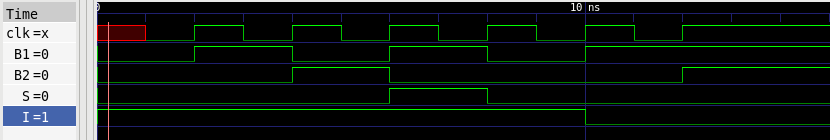
\includegraphics[width=0.7\textwidth]{data/Graficos1/ej1a.png}
    \par\end{centering}
    \caption{Mealy state machine - Verilog test results}
\end{figure}

